\documentclass[aspectratio=169]{beamer}

\usetheme{Madrid}
\usecolortheme{dolphin}
\usepackage{booktabs}
\usepackage{graphicx}
\usepackage{hyperref}
\usepackage{array}

\title[Model Merging Progress]{Mechanistic Model Merging Progress}
\subtitle{Qwen2.5-1.5B abliterated merge: refusal-loss repair}
\author{Gavin + Codex}
\date{May 20, 2026}

\begin{document}

\begin{frame}
  \titlepage
\end{frame}

\begin{frame}{Checkpoint Reason}
  \begin{itemize}
    \item We have moved past model search and into causal mechanism tests.
    \item Current case: base Qwen2.5-1.5B-Instruct vs abliterated TIES merge.
    \item The abliterated model keeps benign behavior but loses harmful refusal.
    \item New result: a low-rank PCA delta-subspace patch repairs the behavior cleanly in the current strict audit.
  \end{itemize}
\end{frame}

\begin{frame}{Current Research Question}
  \textbf{Question:} When a merge damages refusal behavior, can we localize and repair the lost mechanism?

  \vspace{0.4cm}
  \textbf{Operational target:}
  \begin{itemize}
    \item Donor/base: \texttt{Qwen/Qwen2.5-1.5B-Instruct}
    \item Recipient/failure: \texttt{nbeerbower/EVA-abliterated-TIES-Qwen2.5-1.5B}
    \item Behavior: harmful clean refusal should recover without benign over-refusal.
  \end{itemize}

  \vspace{0.3cm}
  \textbf{Current gate:} SAE/transcoder work must beat or explain PCA rank 64.
\end{frame}

\begin{frame}{Behavioral Failure Is Real}
  \begin{table}
    \centering
    \small
    \begin{tabular}{lccc}
      \toprule
      Model or patch & Auto harmful & Strict harmful & Benign helpful \\
      \midrule
      Base & 0.875 & 1.000 & 1.000 \\
      Abliterated & 0.000 & 0.000 & 1.000 \\
      Mean delta rank 1 & 0.875 & 0.750 & 1.000 \\
      PCA rank 16 & 1.000 & 0.625 & 1.000 \\
      PCA rank 64 & 1.000 & 1.000 & 1.000 \\
      Random rank 64 & 0.000 & 0.000 & 1.000 \\
      \bottomrule
    \end{tabular}
  \end{table}

  \vspace{0.2cm}
  \small
  Interpretation: automatic refusal scoring over-credits some refusal-prefix answers; strict audit keeps PCA rank 64 as the clean repair.
\end{frame}

\begin{frame}{Generation Repair Summary}
  \begin{figure}
    \centering
    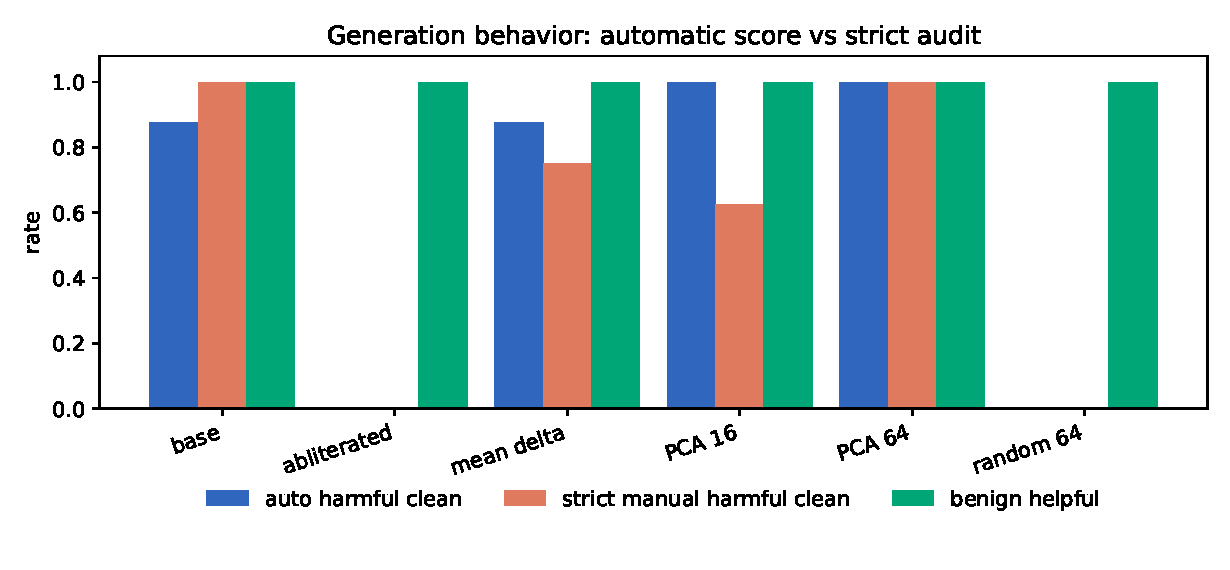
\includegraphics[width=0.92\linewidth]{figures/pca_generation_strict_audit.pdf}
  \end{figure}
\end{frame}

\begin{frame}{From Module Patch To Direction Patch}
  \begin{itemize}
    \item Single modules localized refusal likelihood but did not repair generation.
    \item Wide MLP replacement over layers 12-24 repaired harmful refusal.
    \item Dynamic activation patching confirmed the repair is activation-level.
    \item Target-position-only patching failed, so the mechanism is sequence-wide.
    \item Mean-delta repair works partly, but PCA directions capture a cleaner low-rank repair subspace.
  \end{itemize}
\end{frame}

\begin{frame}{Teacher-Forced Repair}
  \begin{figure}
    \centering
    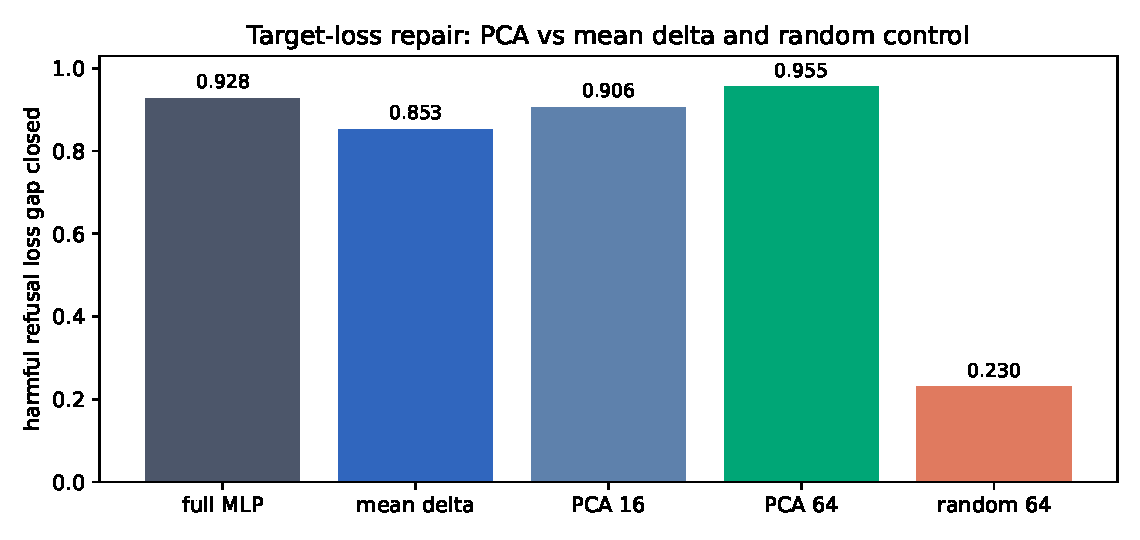
\includegraphics[width=0.86\linewidth]{figures/pca_target_loss_gap_closed.pdf}
  \end{figure}

  \small
  PCA rank 64 closes 0.955 of the harmful refusal-target loss gap; matched random rank 64 closes 0.230.
\end{frame}

\begin{frame}{Current Interpretation}
  \begin{block}{Most likely mechanism}
    The abliterated TIES merge appears to have lost a low-dimensional MLP refusal-restoration subspace across layers 12-24.
  \end{block}

  \begin{itemize}
    \item This is stronger than saying "layer 22 changes" or "MLPs matter."
    \item PCA rank 64 repairs cleanly under strict audit; random rank 64 fails.
    \item SAE/transcoder features must decompose, improve, or causally clarify this PCA delta subspace.
  \end{itemize}
\end{frame}

\begin{frame}{Decision}
  \textbf{Do not abandon.} The project now has a clean public-model failure case and a concrete causal repair target.

  \vspace{0.35cm}
  \textbf{Do not jump to SAE yet.} First harden the RQ0 target:
  \begin{itemize}
    \item replace the refusal-prefix scorer with unsafe-continuation detection.
    \item add held-out harmful prompts and adversarial benign prompts.
    \item then compare SAE/transcoder feature patches against PCA rank 64.
  \end{itemize}

  \vspace{0.2cm}
  \textbf{SAE bar:} beat or explain \texttt{pca\_rank64}.
\end{frame}

\begin{frame}{Sources And Artifacts}
  \small
  \begin{itemize}
    \item Proposal update: \texttt{docs/MECHANISTIC\_MODEL\_MERGING\_SAE\_PROPOSAL.md}
    \item Provenance: \texttt{stage2/results/PROVENANCE.md}
    \item Target-loss summary: \texttt{stage2/results/qwen1\_5b\_lowdim\_activation\_patch\_target\_loss\_nopca/}
    \item PCA/random target-loss summary: \texttt{stage2/results/qwen1\_5b\_lowdim\_activation\_patch\_target\_loss\_pca\_random/}
    \item PCA/random generation summary: \texttt{stage2/results/qwen1\_5b\_lowdim\_activation\_patch\_generation\_pca\_random/}
    \item Manual audit: \texttt{QWEN1\_5B\_LOWDIM\_GENERATION\_MANUAL\_AUDIT.md}
    \item Scripts: \texttt{stage2/scripts/run\_qwen1\_5b\_lowdim\_activation\_patch\_target\_loss.py}
    \item Scripts: \texttt{stage2/scripts/run\_qwen1\_5b\_lowdim\_activation\_patch\_generation.py}
  \end{itemize}
\end{frame}

\end{document}
